\subsection*{QR-Code}
%Herkunft und Nutzung
Der QR-Code wurde 1994 von der japanischen Firma Denso Wave inc., einer Tochterfirma von Toyota, als 'Quick Response Code' entwickelt. Ein Code kann maximal 7089 Ziffern bzw. 4296 Zeichen+Ziffern verschlüsseln und besitzt eine hohe Fehlerkorrekturrate von bis zu 30 \%. Er wird inzwischen in allen Bereichen des täglichen Lebens genutzt, was z.B. auch eine Studie aus dem August 2006 in Japan belegt, wo 82.4\% der zufällig Befragten ihre Handys dafür nutzten QR-Codes zu lesen.(cite{Furht2011})
\todo{Quelle vervollständigen}

%Aufbau
Ein QR-Code besteht aus 5 verschiedenen Bereichen: dem Suchraster, dem Ausrichtungsraster, dem Kalibrierungsraster, der Ruhezone und dem Datenbereich. Das Suchraster besteht aus 3 Quadraten, durch die man die Position, den Drehwinkel und die Größe des Codes ermitteln kann. Das Ausrichtungsraster, ab Version 2, hilft beim Ausgleich von nicht-linearen Verzerrungen. Alle Datensymbole können mit Hilfe des Kalibrierungsraster's gefunden werden. Die Ruhezone, die den Code umgibt, ist für das Finden des Codes, z.B innerhalb eines Bildes, unbedingt nötig und im Datenbereich befinden sich jegliche Daten, die als quadratische Matrix gespeichert werden. Die Codes existieren in 40 verschiedenen Versionen, die die Größe der Matrix festlegen (von 21x21 bis 177x177 Pixel).

Im Datenbereich sind Informationen horizontal und vertikal verschlüsselt, und für die Fehlerkorrektur gibt es 4 Level, L 7\%, M 15\%, Q 25\%, H 30\%, durch die der Code dann entsprechend größer wird.

%Vorteile/Nachteile und Zusätzliches
Die Vorteile des QR-Codes sind die hohe Verschlüsselungskapazität der Daten (Zeichenanzahl), die kleine Druckgröße, Verschmutzungs- und Schadensresistenz (bis zu 30\% des Schaden's kann durch Level H ausgeglichen werden), die Lesbarkeit unabhängig vom Winkel und die Teilbarkeit in mehrere kleine QR-Codes.

\begin{figure}[H]
  \centering
  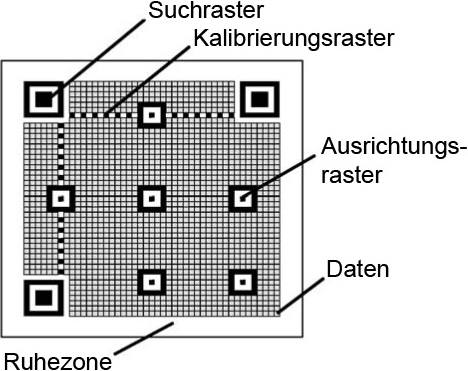
\includegraphics[height=5cm]{img/QR/Aufbau_qr-codes.jpg}
  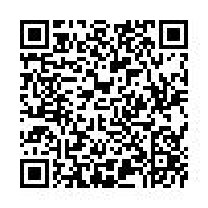
\includegraphics[height=5cm]{img/QR/perfect_03.jpg}
  \caption{Die Bereiche eines QR-Code's und ein Beispielcode}
  \label{fig:qrexample}
\end{figure}

\todo{in Referenzen eingliedern}
%Quellen:
% DensoWave2000-2010: \url{http://www.qrcode.com/en/index.html}
% \url{Site 341 in 'Handbook of Augmented Reality' by Borko Furht}
